\clearpage
\section{Andromeda - Svemirska puca\v{c}ina}
\label{sec:Section_Name_X}

\subsection{Pregled i ideja igre}
Originalna ideja igre je ne\v{s}to \v{s}ira od onoga \v{s}to imamo ovde, tako da \'cemo ovo nazvati demo verzijom. Sa tim na umu
obra\'cena je posebna pa\v{z}nja na to da kod bude lako pro\v{s}iriv, te da nemamo tesne veze izme\dj u klasa, a posebna je vo\dj eno
ra\v{c}una o tome da se sami podaci o aktorima u igri (brodovi, svemirska baza) izdvoje kao posebni objekti (videti \ref{sec:scriptobj})
radi lal\v{s}e konfiguracije i pro\v{s}irivosti. Ukratko \'cemo dati pregled najbitnijih stavki igre.

\emph{Igra\v{c}} dobija kontrolu nad jednim svemirskim brodom koji mo\v{z}e da se kre\'ce isklju\v{c}ivo napred, potiskom, 
ali isto tako mo\v{z}e da se okre\'ce oko svoje ose, te je tako omogu\'ceno kretanje u svim pravcima u ravni. Pored kretanja,
igra\v{c} ima mogu\'cnost da puca na neprijatelje. Tasteri koji se koriste prilikom ovih akcija su strelice, i to \emph{UpArrow} za potisak,
\emph{LeftArrow} i \emph{RightArrow} za rotaciju, i \emph{LeftControl} za pucanje.

\emph{Neprijatelji} su brodovi kontrolisani od strane ra\v{c}unara koji za cilj imaju da uni\v{s}te glavnu
bazu u igri nazvana \emph{Starbase}. U prvoj verziji postoje dve vrste neprijatelja \v{c}iji opisi se nalaze
dalje u tekstu.

\emph{Fighter} ili lovac je mali okretan brod koji napada isklu\v{c}ivo igra\v{c}a. Neprijatelj \v{s}alje
gomilu lovaca kako bi za\v{s}titio napada\v{c}e i ote\v{z}ao odbranu svemirske baze za igra\v{c}a.

\emph{Attacker} ili napada\v{c} je sporiji brod lo\v{s}ijih manevarskih sposobnosti poslat sa ciljem da napada
isklju\v{c}ivo svemirsku bazu. Iako sporiji i manje okretljivi od lovaca ovi brodovi opremljeni su jakim topovima
koji su u mogu\'cnosti da raznesu svemirsku bazu i nanesu ogromnu \v{s}tetu igra\v{c}u ukoliko se nadje
na njihovoj putanji.

\begin{center}
    \begin{figure}
        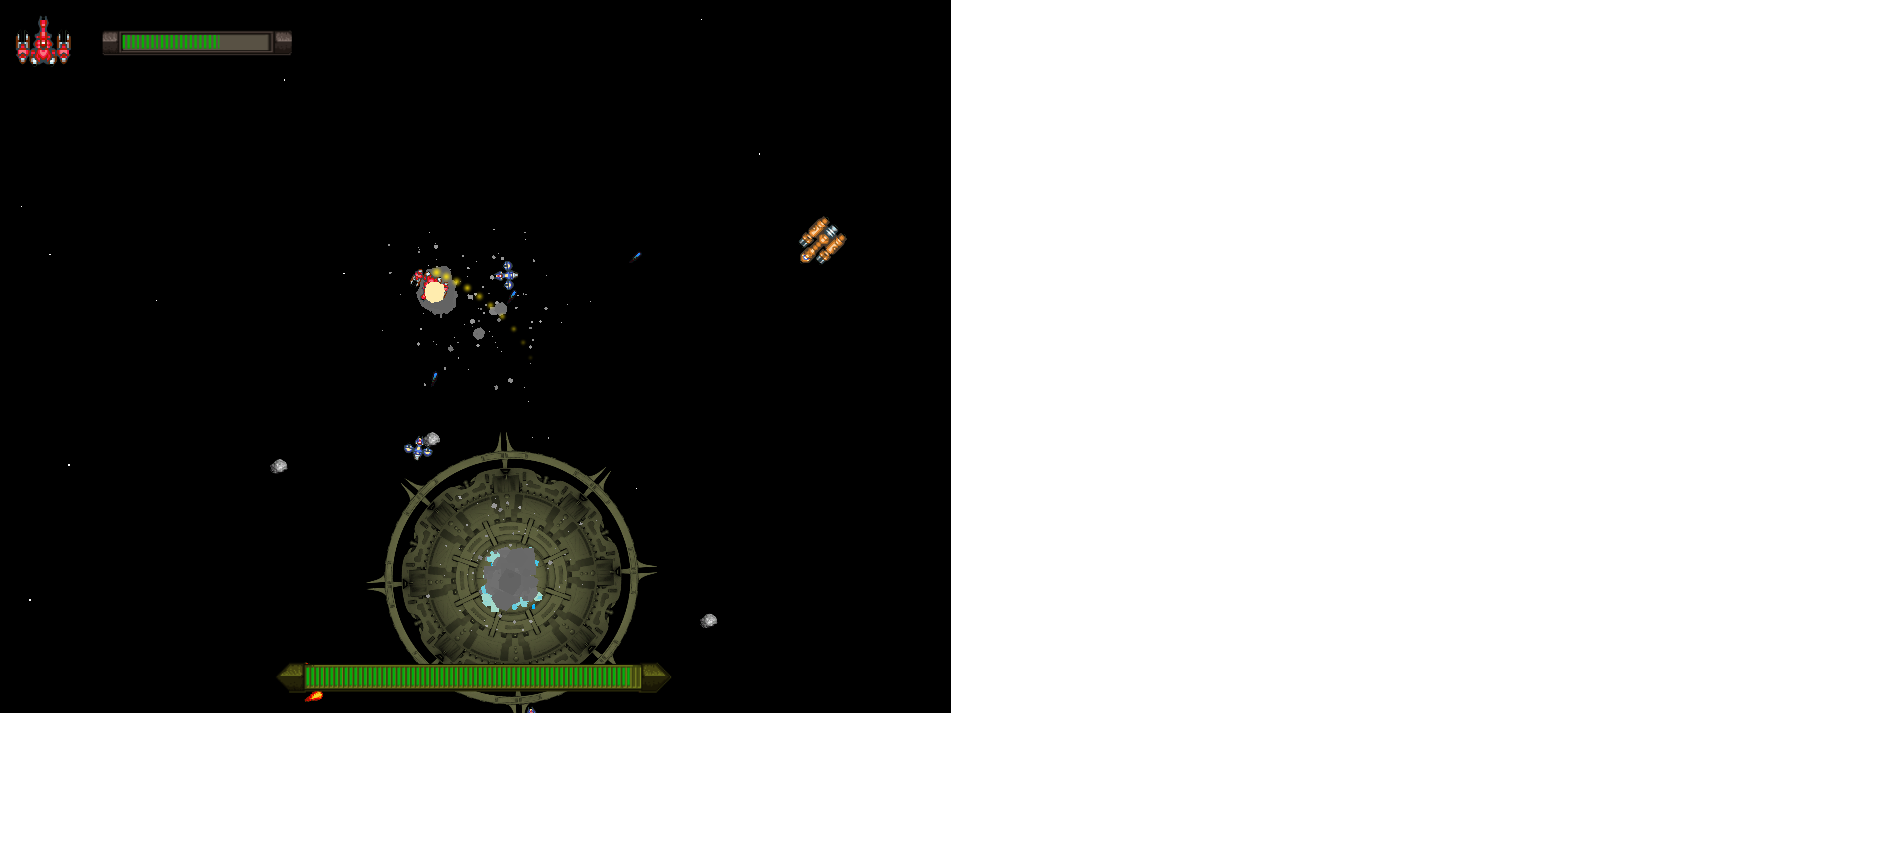
\includegraphics[width=2\textwidth]{Figures/GameScr_01.png}
        \caption{Igra}
        \label{fig:gamescr_01}
    \end{figure}
\end{center}


\subsection{GameManager klasa}
\label{gamemanager}
Ve\'c je bilo re\v{c}i o tome da je ova klasa Singleton odnosno, preciznije, MonoSingleton. Ova klasa zadu\v{z}ena je da
vodi ra\v{c}una o stanju igre. U na\v{s}em slu\v{c}aju, uzev\v{s}i u obzir da je ovo tek demo, ona ne radi puno stvari u ovom trenutku.

\pagebreak

\begin{verbatim}
public sealed class GameManager : MonoSingleton<GameManager>
{
    [SerializeField]
    private GameObject _pnGameOver;
    [SerializeField]
    private GameObject _pnStartGame;

    public int gameWorldRadius = 300;

    private void Start()
    {
        _pnGameOver.SetActive(false);
        _pnStartGame.SetActive(true);
        Time.timeScale = 0;
    }

    public void GameOver(float secs = 0f)
    {
        StartCoroutine(Delay(secs));
    }

    public void StartGame()
    {
        _pnGameOver.SetActive(false);
        _pnStartGame.SetActive(false);
        Time.timeScale = 1;
    }

    private IEnumerator Delay(float secs)
    {
        yield return new WaitForSeconds(secs);
        _pnGameOver.SetActive(true);
        Time.timeScale = 0;
    }

    public void Retry()
    {
        SceneManager.LoadScene(SceneManager.GetActiveScene().buildIndex);
        Destroy(this.gameObject);
    }
}
\end{verbatim}

Dakle, za sada vodi ra\v{c}una o aktivnim ekranima, po\v{c}etku igre i restartovanju nivoa nakon izgubljene igre.
Funkcija \emph{GameOver} zapada za oko, i vidimo da poziva fukciju \emph{StartCoroutine} kojoj kao argument prosle\dj uje
funkciju koja zapravo radi ono \v{s}to treba da se desi kada se igra zavr\v{s}i. Ovo je i razlog za\v{s}to ova klasa
ne mo\v{z}e da bude prosto stati\v{c}ka. Da bismo mogli da pozovemo \emph{korutinu} \ref{sec:coroutines} klasa mora da nasledi
MonoBehaviour, ali nam je istovremeno potreban jednostavan globalan pristup za ovu klasu, jer ho\'cemo da mo\v{z}emo da
zavr\v{s}imo igru sa vi\c{s}e mesta, recimo iz klase koja kontroli\v{s}e igra\v{c}a ili iz klase koja predstavlja 
svemirsku bazu. Odlaganje poziva ovde radimo kako bismo dali trenutak igra\v{c}u da ukapira \v{s}ta se desilo, i za\v{s}to
je igra zavr\v{s}ena. Ovo odlaganje omogu\'cava igra\v{c}u da vidi eksploziju baze ukoliko je to uzrokovalo kraj igre.

Uloga ove klase je dosta \v{s}ira jednom kada igra po\v{c}ne da izlazi iz demo faze i po\v{c}ne da dobija neku celinu. Recimo,
ova klasa vodila bi ra\v{c}una i nivoima u igri, poenima igra\v{c}a, ostalim ekranima koji se smenjuju iz menija pa do glavne scene igre i sli\v{c}no.

\emph{GameOver} zavr\v{s}ava igru tako \v{s}to postavlja timeScale na 0 \v{c}ime prestaje proticanje
vremena u igri \v{s}to zaustavlja sve elemente igre. Pri ponovnom startovanju igre ovo vreme se vra\'ca na prvobitnu vrednost 1.

\subsection{Kontrole i InputManager}
Ova klasa predstavlja blagu apstrakciju za procesiranje korisni\v{c}kog unosa. Jedina stvar koja nam treba zapravo
jeste da unos pretvorimo u niz komandi, koja tako\dj e treba da zna stanje tipke. Stanje defini\v{s}emo pomo\'cu enuma:

\begin{verbatim}
    public enum KeyState
    {
        NONE,
        PRESSED,
        HELD
    }
\end{verbatim}

\begin{verbatim}
public sealed class InputManager : MonoSingleton<InputManager>
{
    public Dictionary<KeyCode, ACommand> InputMap 
        { get; 
        private set; } = new Dictionary<KeyCode, ACommand>();

    public Queue<ACommand> GetInput()
    {
        Queue<ACommand> inputQueue = new Queue<ACommand>();

        foreach (var input in InputMap)
        {
            // Down
            if (Input.GetKeyDown(input.Key))
            {
                input.Value.State = KeyState.PRESSED;
                inputQueue.Enqueue(input.Value);
            }

            // Pressed
            else if (Input.GetKey(input.Key))
            {
                input.Value.State = KeyState.HELD;
                inputQueue.Enqueue(input.Value);
            }
        }

        return inputQueue;
    }
}
\end{verbatim}

InputMap smo videli ve\'c kada smo pri\v{c}ali o \emph{Command} obrascu, a ovde sada vidimo celu funkciju
\emph{GetInput} koja vra\'ca niz komandi kroz strukturu \emph{Queue} radi lak\v{s}e obrade i o\v{c}uvanja redosleda.
Imamo dve vrste registrovanja pritiska tipke sa tastature: tipka je pritisnuta i tipka je zadr\v{z}ana. Ovo nam je bitno,
jer recimo ho\'cemo da igra\v{c} mora konstantno da pritiska tipku ako ho\'ce da puca, a to isto bi bilo dosta
naporno raditi za kretanje, tako da je za kretanje dovoljno da je tipka zadr\v{z}ana.

\subsection{Pona\v{s}anje svemirskog broda i ShipController klasa}
\emph{ShipController} klasa je klasa koja opisuje pona\v{s}anje broda u op\v{s}tem slu\v{c}aju, dakle ovu klasu 
u osnovi koriste i neprijatelji i igra\v{c}. Ova klasa obra\dj uje komande (akcije) kroz glavnu petlju igre, odnosno
u funkciji \emph{FixedUpdate} u kojoj se izvr\v{s}avaju sve akcije koje uti\v{c}u na fiziku. Akcije dodajemo
u red.

\begin{verbatim}
protected Queue<ACommand> actions = new Queue<ACommand>();
public void AddAction(ACommand action) => actions.Enqueue(action);
\end{verbatim}

Ove akcije dalje procesiramo:

\begin{verbatim}
protected void FixedUpdate()
{
    while (actions.Count > 0)
    {
        var action = actions.Dequeue();
        action.Execute(this, _actor);
    }
}
\end{verbatim}

Ostatak klase bavi se samim pomeranjem kao i detekcijom kolizije. Ono \v{s}to je jo\v{s} bitno
napomenuti jeste da se klasa oslanja na \emph{ScriptableObjects} za konfiguraciju, tako vidimo definiciju 
polja tipa \emph{Actor} i \emph{ActorConfig} na osnovu kojeg se zapravo pravi sam \emph{Actor}. \emph{ActorConfig} je
apstrakcija podataka i definisan je kao \emph{ScriptableObject}. Prilo\v{z}ene su obe klase:

\begin{verbatim}
    [CreateAssetMenu(fileName = "Actor", 
        menuName = "Andromeda/Ships/ActorConfig", order = 1)]
    public class ActorConfig : ScriptableObject
    {
        public int HitPoints;
        public float ThrustPower;
        public float RotationCoef;
    }

    public class Actor
    {
        public int HitPoints;
        public float ThrustPower;
        public float RotationCoef;

        public Actor(ActorConfig config)
        {
            HitPoints = config.HitPoints;
            ThrustPower = config.ThrustPower;
            RotationCoef = config.RotationCoef;
        }
    }
\end{verbatim}

\begin{verbatim}
public class ShipController : MonoBehaviour
{

    public ActorConfig config;
    protected Actor _actor;

    public void AddThrust(Vector2 direction, float force)
    {
        if (GetComponent<Rigidbody2D>().velocity.magnitude > 
            maxVelocity)
        {
            Debug.Log("Already at max speed");
            return;
        }

        GetComponent<Rigidbody2D>().AddForce(direction * force);
    }

    public void AddRotation(float rotation)
    {
        transform.Rotate(Vector3.forward, 
            rotation * Time.deltaTime);
    }

    protected void OnTriggerEnter2D(Collider2D collider)
    {
        if (collider.gameObject.tag.Equals("Projectile"))
        {
            var ammo = 
                collider.gameObject
                .GetComponent<Projectile>()
                .GetAmmoConfig;
            _actor.HitPoints -= ammo.Damage;

            // Check death
            if (_actor.HitPoints <= 0)
            {
                // Died
                if (OnDeath != null)
                {
                    // Custom death event
                    OnDeath();
                }
                else
                {
                    // Default death event
                    // TODO: avoid dynamic allocation
                    Instantiate(destroyedParticles, 
                        transform.position, Quaternion.identity);
                    Destroy(this.gameObject);
                }
            }
            else
            {
                // TODO: avoid dynamic allocation
                Instantiate(hitParticles, 
                    transform.position, Quaternion.identity);
            }
        }
    }
}
\end{verbatim}

Ovu klasu nasle\dj uje i \emph{PlayerController} klasa koja dodatno jo\v{s} procesira akcije:

\begin{verbatim}

public sealed class PlayerController : ShipController
{
    ...

    private void Update()
    {
        var inputs = InputManager.Instance.GetInput();
        while (inputs.Count > 0)
        {
            var action = inputs.Dequeue();
            if (!action.IsPhysics)
            {
                action.Execute(this, _actor);
            }
            else
            {
                this.AddAction(action);
            }
        }

        if (transform.position.sqrMagnitude >= 300f)
        {
            Debug.LogWarning("Game Over out of range!");
        }
    }

    ...
}
\end{verbatim}

U zavisnosti od toga da li akcije uti\v{c}u na fiziku, procesiraju se direktno, ili se delegiraju u red akcija
koje procesira ShipController klasa u FixedUpdate.

\subsection{Neprijatelji i osnovno pona\v{s}anje}
Neprijatelji su skriptovani krajnje jednostavno, sa svega dve akcije koje izvr\v{s}avaju: pomeraj se ka meti, pucaj na metu, stoga nije 
bilo potrebe za kompleksnijim pristupom skriptovanja AI pona\v{s}anja. Jedan od takvih pristupa jeste tzv. \emph{stablo pona\v{s}anja} (eng. 
behavior tree) ali se ovime ne\'cemo baviti. Pona\v{s}anja neprijatelja skriptovana su u Update funkciji. Date su Update funkcije
koje opisuju pona\v{s}anje obe vrste neprijatelja. Uo\v{c}avamo da se ne razlikuju su\v{s}tinski.

\begin{verbatim}
// Attacker
private new void Update()
{
    base.Update();

    // Target does not exist
    if (!_starbase) return;

    // Move towards
    Vector2 targetDir = 
        _starbase.transform.position - transform.position;

    // Rotate towards
    float dot = 
        Vector2.Dot(transform.right, targetDir) + 0.5f;

    if (Mathf.Abs(dot) > float.Epsilon)
    {
        actions.Enqueue(new Rotate(-dot));
    }

    if (targetDir.magnitude >= 10f)
    {
        actions.Enqueue(new Thrust());
    }
    else
    {
        // Close enough to shoot
        if (Time.time - _lastFire > fireRate)
        {
            _lastFire = Time.time;
            actions.Enqueue(
                new AIShoot(Ship.Ammo.AmmoType.ROCKET, _guns));
        }
    }
}
\end{verbatim}

\begin{verbatim}
// Fighter
private new void Update()
{
    base.Update();

    // Move towards
    Vector2 targetDir = _target.position - transform.position;
    if (targetDir.magnitude >= 5f)
    {
        actions.Enqueue(new Thrust());
    }

    // Face target
    float dot = Vector2.Dot(transform.right, targetDir) + 0.5f;
    if (Mathf.Abs(dot) > float.Epsilon)
    {
        actions.Enqueue(new Rotate(-dot));
    }

    // Shoot
    if (targetDir.magnitude <= 15f && 
        Time.time - _lastFire >= fireRate)
    {
        _lastFire = Time.time;
        actions.Enqueue(
            new AIShoot(Ship.Ammo.AmmoType.DEFAULT_AI, _guns));
    }
}
\end{verbatim}

\pagebreak
\subsection{Zaklju\v{c}ak}

Pojedini detalji oko kori\v{s}\'cenja funkcija koje daje Unity platforma nisu obja\v{s}njeni jer se iz konteksta
mo\v{z}e zaklju\v{c}iti kada se koriste. Detalje je mogu\'ce lako prona\'ci na sajtu dokumentacije pretragom po imenu
klase ili funkcije. 

Za kompletnu implementaciju pogledati repozitorijum na \href{http://github.com/rtojagic/andromeda}{github.com}. 
Verzija kori\v{s}\'cena za izradu ovog projekta jeste \emph{Unity 2019.4.9f1 Personal}.